\documentclass[11pt]{amsart}
%%% WARNING: Do NOT change the page size, fonts, or margins!  Penalties will apply.


\usepackage{graphicx}
\usepackage{amssymb,amsmath,amsthm, mathtools}
\usepackage{placeins} %enables \FloatBarrier, that prevents floats from going below it.
\usepackage{caption}
\usepackage{subcaption}
\usepackage{algpseudocode, algorithm}
\usepackage{tikz}
\usepackage{physics}
\usetikzlibrary{arrows}
\usetikzlibrary{tikzmark}

%%% WARNING: Do NOT change the page size, fonts, or margins!  Penalties will apply.
%%% WARNING: Do NOT change the page size, fonts, or margins!  Penalties will apply.

% Some macros for ease of use
\newcommand{\R}{{\mathbb R}}
\newcommand{\A}{{\mathrm{A}}}


\begin{document}

\title{Angle approximation from pressure measurements}
\author{Cannon Tuttle, Curtis Evans, Spencer Ashton, Tyler Sanders}

%% comment out next command to put today's date after names of group members, or put a desired day in the parethesis
\date{}

\maketitle

\begin{abstract}
    
\end{abstract}

%% First Section
\section{Problem Statement and Motivation}
A BYU Acoustics Research Group project is currently using a microphone array and triangulation to calculate the direction of arrival of a 
source in relation to the center of the array. They’ve implemented some rudimentary filtering, but so far the results of the calculation are 
somewhat unreliable. We want to take this process and model it as a time series/Hidden Markov model in order to optimize the calculation process. 
We will potentially employ Kalman filtering in order to filter angle measurements. We will also explore whether cross-correlation or GCC-PHAT 
is the better measure of coherence between microphone signals for this purpose, and whether the hidden state should be modeled as an angle or 
be modeled directly as a series of coherence measurements. We will also experiment with ways to represent the observation space. This will also 
include trying to predict whether there is or isn’t a speaker currently present.


Several of the noise reduction algorithms they have implemented depend on a highly accurate angle measurement. As those algorithms have already been 
implemented, we would be primarily concerned with the step of direction of arrival angle estimation and optimization, as well as optimally estimating 
the corresponding time delay. This would provide the research group with enhanced measurements for use in their noise processing algorithms.
	

This relates to the hidden markov model because we don’t know what the angles are that we are looking for, but we do know how to take a measurement of 
the current pressure at each microphone. We will use these microphones to be our observed data to then figure out what these angles are by creating a HMM. 
The angles are to be calculated at discrete time steps according to the current pressure measurement. The Kalman filter might accurately represent the 
system and more optimally combine current and prior information about the angle in order to calculate a less noisy current angle estimate.

%% Second Section
\section{Data}
The data for this project will be provided by the research team (Curtis Garner) that is currently working on it. The data includes measurements where the sound 
source is and is not moving, is and is not present, and measurements that do and don’t include machine noise in the microphone signal.




%% Third Section 
\section{Methods}
We have tried several methods to compute the hidden angle measurement. We tried the following methods...

\subsection{State Space Model}
First we had to set up our continuous state space model. We chose the following set up
\[\mathbf{x}_t = \begin{pmatrix*}[l]
    \theta_t \\
    \theta_{t-1} \\
    \theta'
\end{pmatrix*},\;  
F = \begin{pmatrix*}[l]
    1 & 0 & \Delta t \\
    1 & 0 & 0 \\
    \frac{1}{\Delta t} & \frac{1}{\Delta t} & 0
\end{pmatrix*},\;
H = \begin{pmatrix*}[l]
    1 & 0 & 0 \\
    \vdots & \vdots & \vdots\\
    1 & 0 & 0

\end{pmatrix*}\]
 where $H$ is of dimension $18\times3$. We don't have any control in our situation so our state space is
 \[\mathbf{x}_t = F\mathbf{x}_{t-1} + \mathbf{w}_t,\]
\[\mathbf{z}_t = H\mathbf{x}_t + \mathbf{v}_t\].

\subsection{Kalman Filter}
We implemented an extended version of the Kalman filter \cite{V3} and with stimulated data like done in the lab manuals we were struggling 
to get the wraparound from angles in the range of \[2\pi - \epsilon \leq \theta \leq 2\pi + \epsilon.\] See figure \ref{fig:simple_kalman}
to get a visual.

We discovered that the problem was occurring in the update step where \[\mathbf{\tilde{y}}_k = \mathbf{z}_k - H\mathbf{\hat{x}}_{k|k-1}\]
so we figured out the best way to fix this was to implement Algorithm \ref{alg:kalman}. We saw great results from this in our stimulated data.
See Figure \ref{fig:simple_kalman}.

\begin{figure}[htp]
    \centering
    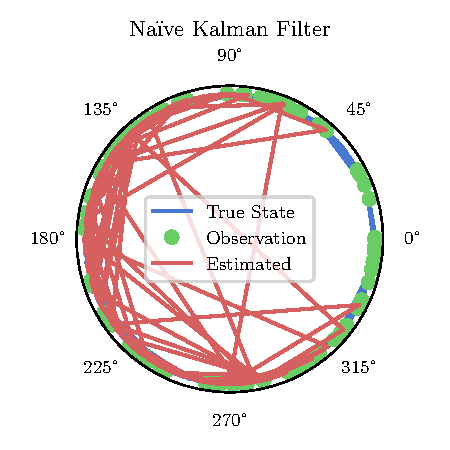
\includegraphics[width=0.47\textwidth]{non_altered_kalman.pdf}\hfill
    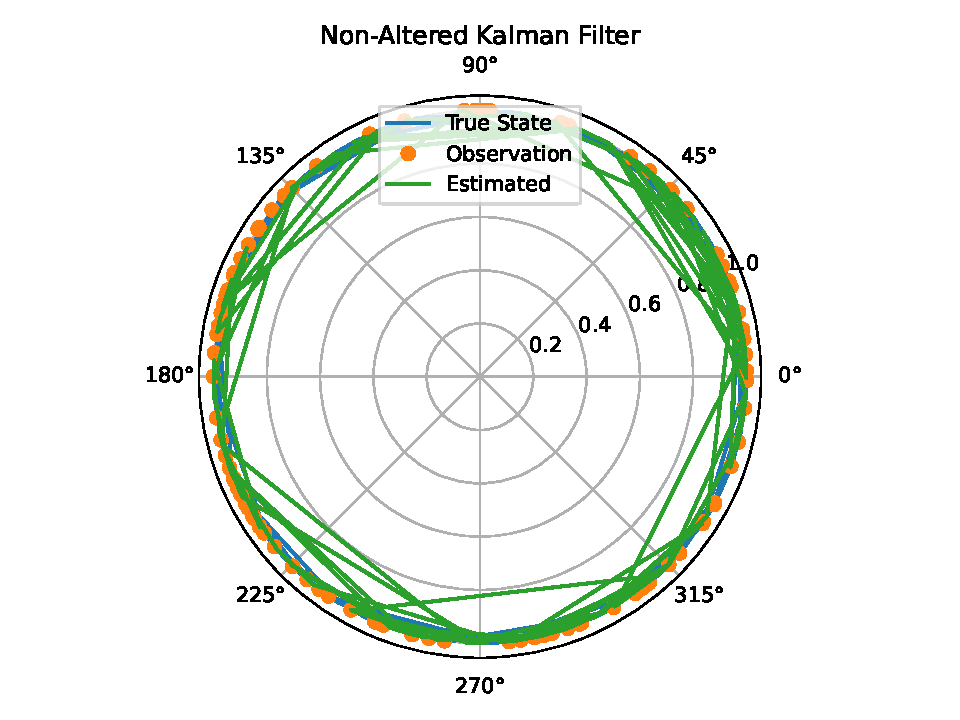
\includegraphics[width=0.47\textwidth]{altered_kalman.pdf}\hfill
    \caption{The altered and non-altered Kalman Filter}
    \label{fig:simple_kalman}
\end{figure}



\begin{algorithm}
    \caption{Process to Fix Wraparound}\label{alg:kalman}    
    \begin{algorithmic}
        \If{$\lvert{\mathbf{z_k} - H\mathbf{x_k}}\rvert \geq \pi \;\textbf{and}\; \mathbf{z_k} \leq 0$} 
            \State $\mathbf{z_k} \gets \mathbf{z_k} + 2\pi$
        \ElsIf{$\lvert{\mathbf{z_k} - H\mathbf{x_k}}\rvert \geq \pi \;\textbf{and}\; \mathbf{z_k} \geq 0$} 
            \State $\mathbf{z_k} \gets \mathbf{z_k} - 2\pi$
        \EndIf 
        \end{algorithmic}
    \end{algorithm}

%% Insert some pictures of the angle adjustment and add the algorithm 

\subsection{Particle Filter}

\subsection{HMM Model}

\section{Results}

\section{Analysis}

\section{Ethical Considerations}
Some possible use cases of this project would be so that big machinery can detect an angle of danger where a person might be. 
This isn't a great a 

\section{Conclusion}






\begin{figure}[htp]
    \hfill
    \begin{subfigure}[b]{0.32\textwidth}
        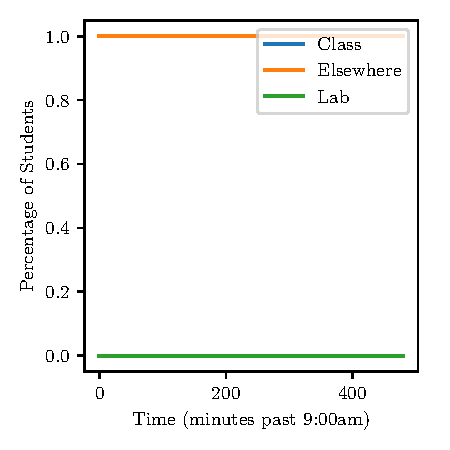
\includegraphics[width=\textwidth]{temp.pdf}
        \caption{$A_{interp.7}$}
        \label{fig:interp_degrees_7}
    \end{subfigure}
    \hfill
    \begin{subfigure}[b]{0.32\textwidth}
        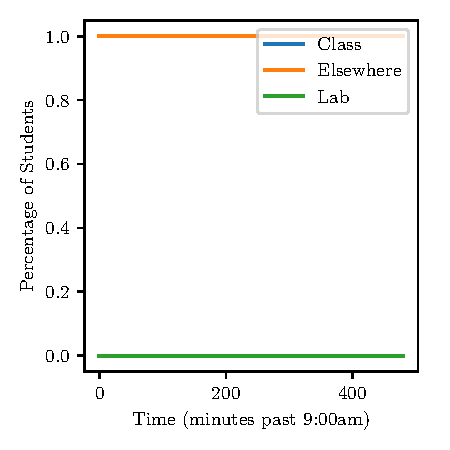
\includegraphics[width=\textwidth]{temp.pdf}
        \caption{$A_{interp.12}$}
        \label{fig:interp_degrees_12}
    \end{subfigure}
    \hfill
    \begin{subfigure}[b]{0.32\textwidth}
        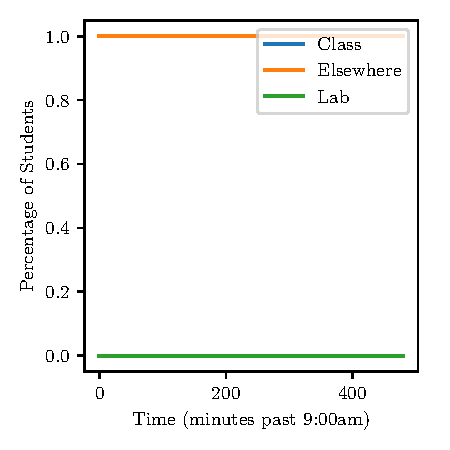
\includegraphics[width=\textwidth]{temp.pdf}
        \caption{$A_{interp.25}$}
        \label{fig:interp_degrees_25}
    \end{subfigure}
    \caption{Continuizing $A_{discontinuous}$ with various degrees of Barycentric Lagrange Interpolation 
    at the Chebyshev points. Our ensuing models use the 12-degree interpolation (bottom-left).}
    \label{fig:interp_degrees}
\end{figure}







\begin{figure}[htp]
    \centering
    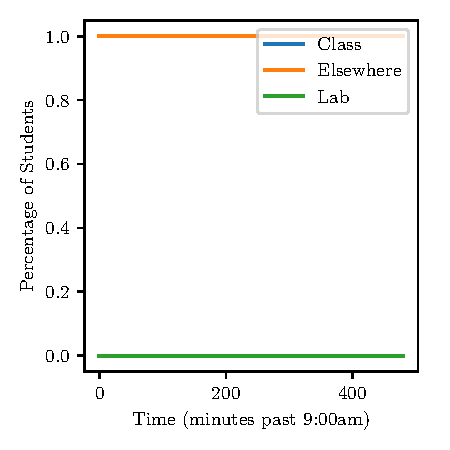
\includegraphics[width=0.45\textwidth]{temp.pdf}\hfill
    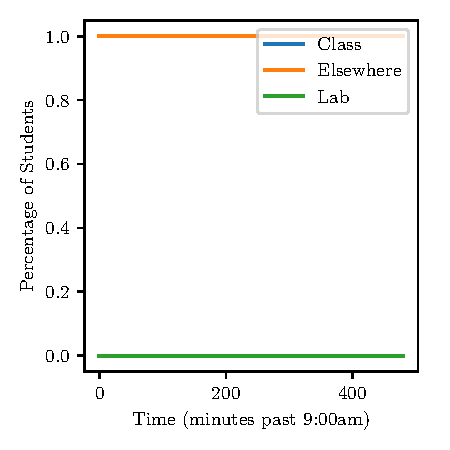
\includegraphics[width=0.45\textwidth]{temp.pdf}\hfill
    \caption{The constant alpha functions (left) along with the timeplot using IVP (right).}
    \label{fig:constant_alpha}

\end{figure}


\begin{figure}[htp]
    \centering
    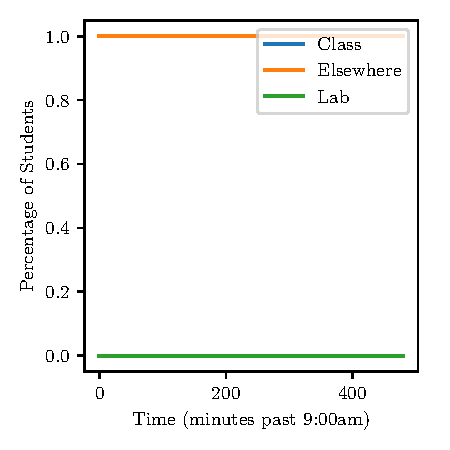
\includegraphics[width=0.45\textwidth]{temp.pdf}\hfill
    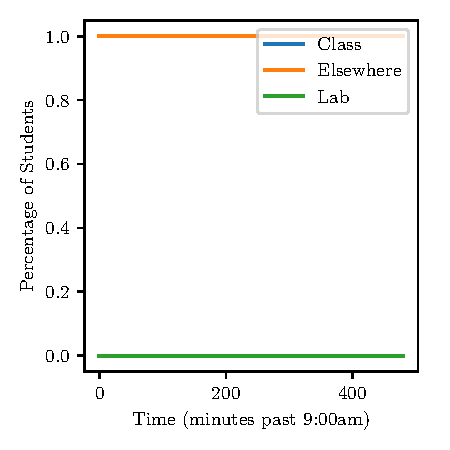
\includegraphics[width=0.45\textwidth]{temp.pdf}\hfill

    \caption{The discontinuous alpha functions (left) along with the timeplot using IVP (right).}
    \label{fig:discontinuous_alpha}

\end{figure}


\begin{figure}[htp]
    \centering
    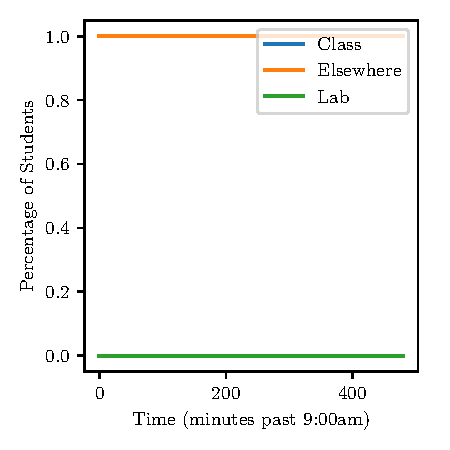
\includegraphics[width=0.5\textwidth]{temp.pdf}
    \caption{Timeplot of our ODE system with $A_{discontinuous}$, but using a BVP solver.}
    \label{fig:discontinuous_alpha_bvp}

\end{figure}



\begin{figure}[htp]
    \centering
    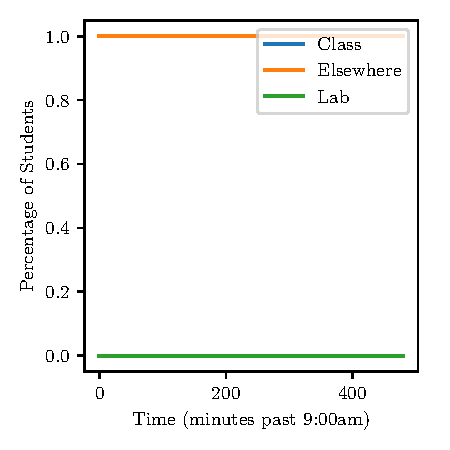
\includegraphics[width=0.3\textwidth]{temp.pdf}\hfill
    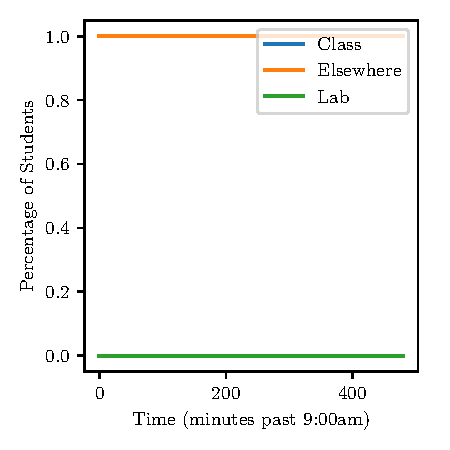
\includegraphics[width=0.3\textwidth]{temp.pdf}\hfill
    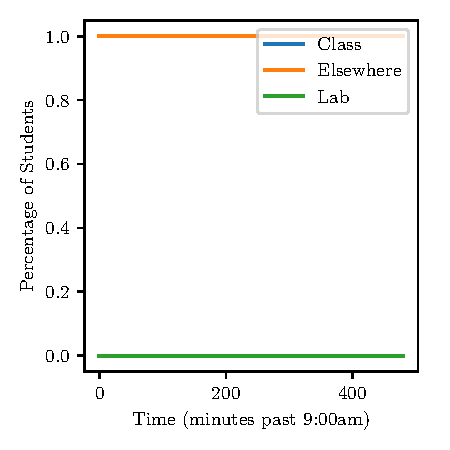
\includegraphics[width=0.3\textwidth]{temp.pdf}\hfill
    \caption{Simulating with $A_{interp.12}$ (left), giving the timeplots using both IVP (center) and BVP (right).}
    \label{fig:continuous_alpha}

\end{figure}


\begin{figure}[htp]
    \centering
    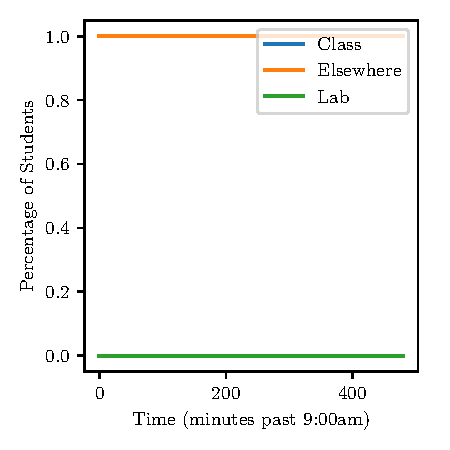
\includegraphics[width=1\textwidth]{temp.pdf}\hfill
    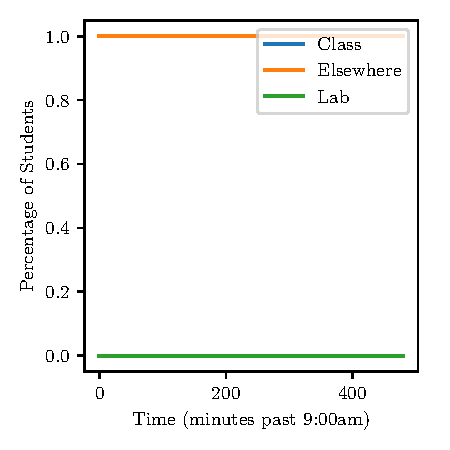
\includegraphics[width=0.45\textwidth]{temp.pdf}\hfill
    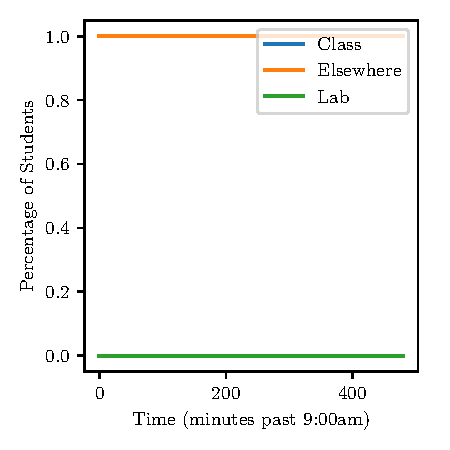
\includegraphics[width=0.45\textwidth]{temp.pdf}\hfill

    \caption{Simulating our IVP with $A_{interp.12}$ plus some gaussian terms for daily traffic (top), along with the timeplot using IVP (bottom-left) and BVP (bottom-right).
    our BVP spikes far outside our usual bounds at transitions with daily traffic.}
    \label{fig:daywise_alpha}
\end{figure}







%%%%%%%%%%%%%%%%%%%%%%%%%%%%%%%%%%%%%
%% Bibliography below
%%%%%%%%%%%%%%%%%%%%%%%%%%%%%%%%%%%%%
\FloatBarrier % Keep the figures from being put after the bibliography
\newpage
%% If using bibtex, leave this uncommented
%\bibliography{refs} %if using bibtex, call your bibtex file refs.bib
\bibliographystyle{alpha}

%% If not using bibtex, comment out the previous two lines and uncomment those below
\begin{thebibliography}{99}
\bibitem{V3} The ACME Volume 3 Textbook
\bibitem{Migration} Wang Xiang-Sheng and Wu Jianhong 2012. Seasonal migration dynamics: periodicity, transition delay and finite-dimensional reductionProc. R. Soc. A.468634–650. http://doi.org/10.1098/rspa.2011.0236
\bibitem{Population} Pierre Auger, Jean-Christophe Poggiale, Emergence of Population Growth Models: Fast Migration and Slow Growth, Journal of Theoretical Biology, Volume 182, Issue 2, 1996, Pages 99-108, ISSN 0022-5193, https://doi.org/10.1006/jtbi.1996.0145.
\end{thebibliography}

\end{document}
